%                      Code_Saturne version 1.3
%                      ------------------------
%
%     This file is part of the Code_Saturne Kernel, element of the
%     Code_Saturne CFD tool.
%
%     Copyright (C) 1998-2007 EDF S.A., France
%
%     contact: saturne-support@edf.fr
%
%     The Code_Saturne Kernel is free software; you can redistribute it
%     and/or modify it under the terms of the GNU General Public License
%     as published by the Free Software Foundation; either version 2 of
%     the License, or (at your option) any later version.
%
%     The Code_Saturne Kernel is distributed in the hope that it will be
%     useful, but WITHOUT ANY WARRANTY; without even the implied warranty
%     of MERCHANTABILITY or FITNESS FOR A PARTICULAR PURPOSE.  See the
%     GNU General Public License for more details.
%
%     You should have received a copy of the GNU General Public License
%     along with the Code_Saturne Kernel; if not, write to the
%     Free Software Foundation, Inc.,
%     51 Franklin St, Fifth Floor,
%     Boston, MA  02110-1301  USA
%
%-----------------------------------------------------------------------
%
%%%%%%%%%%%%%%%%%%%%%%%%%%%%%%%%%%
%%%%%%%%%%%%%%%%%%%%%%%%%%%%%%%%%%
\section{Discr\'etisation} \label{Base_Visort_paragraphe2}
%%%%%%%%%%%%%%%%%%%%%%%%%%%%%%%%%%
%%%%%%%%%%%%%%%%%%%%%%%%%%%%%%%%%%
La figure \ref{Base_Visort_fig_geom} rappelle les diverses d\'efinitions g\'eom\'etriques
pour les faces internes et les faces de bord.

\begin{figure}[h]
\parbox{8cm}{%
\centerline{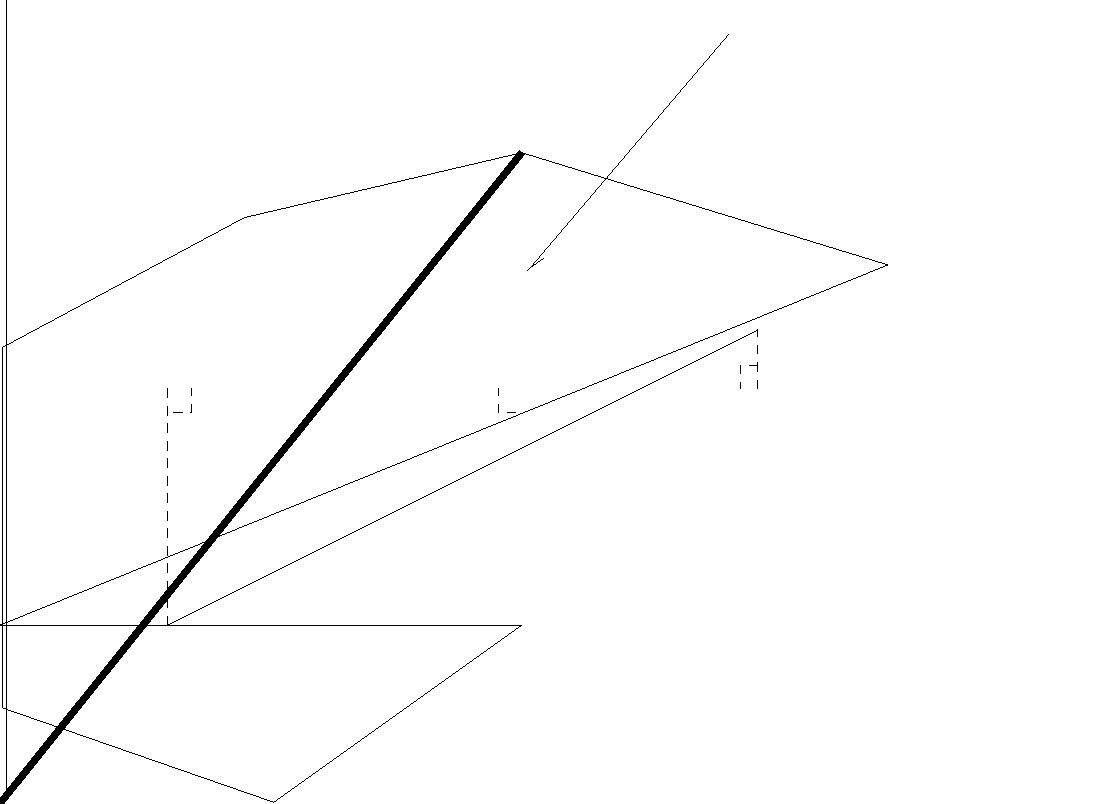
\includegraphics[height=4.5cm]{../Base/Visort/Images/facette.pdf}}}
\parbox{8cm}{%
\centerline{
\includegraphics[height=4.5cm]{../Base/Visort/Images/facebord.pdf}}}
\caption{\label{Base_Visort_fig_geom}D\'efinition des diff\'erentes entit\'es
g\'eom\'etriques pour les faces internes (gauche) et de bord (droite).}
\end{figure}
L'int�gration du terme de diffusion ``orthotrope'' sur une cellule est la
suivante :
\begin{equation}
\int_{\Omega_i}\dive \,(\tens{\mu}\ \grad f)\,d\Omega =\sum\limits_{j \in
Vois(i)}( \tens{\mu}\ \grad f)_{\,ij}\,.\,\underline{S}_{\,ij} + \sum\limits_{k \in
\gamma_b(i)}( \tens{\mu}\ \grad f)_{\,b_{ik}}\,.\,\underline{S}_{\,b_{ik}}
\end{equation}
avec :
\begin{equation}
\tens{\mu}=\begin{bmatrix}\mu_x & 0 & 0 \\ 0 & \mu_y & 0 \\ 0 & 0 & \mu_z \end{bmatrix}
\end{equation}
et :
\begin{equation}
\begin{array}{ll}
&\underline{S}_{\,ij} = S_{\,ij} \underline{n}_{\,ij} \\
&\underline{S}_{\,b_{ik}} = S_{\,b_{ik}} \underline{n}_{\,b_{ik}}
\end{array}
\end{equation}
Le terme $(\tens{\mu}\ \grad(f))_{\,ij}\underline{n}_{\,ij}$ est calcul� �
l'aide de la d�composition suivante :
\begin{equation}
(\tens{\mu}\ \grad f)_{\,ij} = (\grad f \,.\,\underline{n}_{\,ij})\ \tens{\mu}\
\underline{n}_{\,ij}+
(\grad f .\underline{\tau}_{ij})\ \tens{\mu}\ \underline{\tau}_{\,ij}
\end{equation}
o\`u $\underline{\tau}_{ij}$ repr�sente un vecteur tangent (unitaire) �
la face. Une d�composition similaire est utilis�e aux faces de bord.\\
Dans la matrice, seul le terme
$(\grad f \,.\,\underline{n}_{\,ij})\ \tens{\mu}\ \underline{n}_{\,ij}$ est
int\'egrable facilement en implicite. Par cons\'equent, la partie projet\'ee sur $\underline{\tau}_{\,ij}$
est :
\begin{itemize}
\item n\'eglig\'ee dans le cas du calcul des �chelles de temps relatives au
couplage vitesse-pression renforc�,
\item trait\'ee en explicite dans les termes de diffusion de
$R_{\,ij}-\varepsilon$ (\emph{cf.} \fort{turrij}).\\
\end{itemize}
L'int�gration implicite du terme de diffusion s'\'ecrit :
\begin{equation}
\int_{\Omega_i}\dive\,(\tens{\mu}\ \grad f )\,d\Omega = \sum\limits_{j \in
Vois(i)}(\tens{\mu}\ \underline{n}_{\,ij})\,.\,\underline{S}_{\,ij}\,
\frac{f_{J'}-f_{I'}}{\overline{I'J'}} + \sum\limits_{k \in
\gamma_b(i)}(\tens{\mu}\ \underline{n}_{\,b_{ik}})\,.\,\underline{S}_{\,b_{ik}}
\,\frac{f_{\,b_{ik}}-f_{I'}}{\overline{I'F}}
\end{equation}
Dans ce sous-programme, on calcule le terme
$\displaystyle \frac{(\tens{\mu}\
\underline{n}_{\,ij})\,.\,\underline{S}_{\,ij}}{\overline{I'J'}}$ \`a l'aide la
formule :
\begin{equation}\notag
(\tens{\mu}\ \underline{n}_{\,ij})\,.\,\underline{n}_{\,ij} =
\mu_{\,ij}^{\,moy}=\mu_{\,ij}^{\,x} ( n_{\,ij}^{\,x})^2 + \mu_{\,ij}^{\,y} (n_{\,ij}^{\,y})^2 + \mu_{\,ij}^{\,z}(n_{\,ij}^{\,z})^2
\end{equation}
soit encore :
\begin{equation}\notag
\mu_{\,ij}^{\,moy}=\frac{\mu_{\,ij}^{\,x}
(S_{\,ij}^{\,x})^2 + \mu_{\,ij}^{\,y} (S_{\,ij}^{\,y})^2 +
\mu_{\,ij}^{\,z} (S_{\,ij}^{\,z})^2}{S_{\,ij}^2}
\end{equation}
Au bord, on calcule de m�me :
\begin{equation}\notag
\displaystyle \frac{(\tens{\mu}\
\underline{n}_{\,b_{ik}})\,.\,\underline{S}_{\,b_{ik}}}{\overline{I'F}}
\end{equation}

 avec :
\begin{equation}\notag
(\tens{\mu}\ \underline{n}_{\,b_{ik}})\,.\,\underline{n}_{\,b_{ik}} =
\mu_{\,b_{ik}}^{\,moy} = \displaystyle \frac{\mu_{I}^{\,x}
(S_{\,b_{ik}}^{\,x})^2 + \mu_{I}^{\,y} (S_{\,b_{ik}}^{\,y})^2 +
\mu_{I}^{\,z} (S_{\,b_{ik}}^{\,z})^2}{S_{\,b_{ik}}^2}
\end{equation}

La valeur de la viscosit� dans une direction $l$ sur la face, $\mu_{\,ij}^{\,l}$,
est calcul�e :
\begin{itemize}
\item soit par interpolation lin\'eaire :
\begin{equation}
\mu_{\,ij}^{\,l}=\alpha_{\,ij}\mu_{i}^{\,l}+(1-\alpha_{\,ij})\mu_{j}^{\,l}
\end{equation}
avec $\alpha_{\,ij}= 0.5$ car ce choix semble stabiliser bien que cette
interpolation soit d'ordre 1 en espace en convergence,
\item soit par interpolation harmonique :
\begin{equation}\notag
\mu_{\,ij}^{\,l}=\displaystyle
\frac{\mu_{i}^{\,l}\ \mu_{j}^{\,l}}{\alpha_{\,ij}\mu_{i}^{\,l}+(1-\alpha_{\,ij}) \mu_{j}^{\,l}}
\end{equation}
o� :
\begin{equation}\notag
\displaystyle \alpha_{\,ij}=\frac{\overline{FJ'}}{\overline{I'J'}}
\end{equation}
\end{itemize}
